\documentclass{VUMIFPSbakalaurinis}
\usepackage{algorithmicx}
\usepackage{algorithm}
\usepackage{algpseudocode}
\usepackage{amsfonts}
\usepackage{amsmath}
\usepackage{bm}
\usepackage{caption}
\usepackage{color}
\usepackage{float}
\usepackage{graphicx}
\usepackage{listings}
\usepackage{subfig}
\usepackage{wrapfig}
\usepackage[table,xcdraw]{xcolor}
\usepackage{enumitem}
\usepackage{longtable}
\setitemize{noitemsep,topsep=0pt,parsep=0pt,partopsep=0pt}
\setenumerate{noitemsep,topsep=0pt,parsep=0pt,partopsep=0pt}

\hbadness=100000
% Titulinio aprašas
\university{Vilniaus universitetas}
\faculty{Matematikos ir informatikos fakultetas}
\department{Programų sistemų studijų programa}
\papertype{Mokslo tiriamasis darbas III}
\title{Srautinio apdorojimo sistemų balansavimas taikant mašininį mokymąsi}
\titleineng{Balancing stream processing systems using machine learning}
\author{Vytautas Žilinas}
\supervisor{Andrius Adamonis}
\reviewer{Prof. dr. Aistis Raudys}
\date{Vilnius – \the\year}

% Nustatymai
% \setmainfont{Palemonas}   % Pakeisti teksto šriftą į Palemonas (turi būti įdiegtas sistemoje)
\bibliography{bibliografija}

\begin{document} 
\maketitle

\cleardoublepage\pagenumbering{arabic}
\setcounter{page}{2}

\tableofcontents

\sectionnonum{Įvadas}

Realaus laiko duomenų apdorojimas (angl. real–time data processing) yra jau senai nagrinėjamas kaip vienas iš būdų apdoroti didelių kiekių duomenis (angl. Big data). Viena iš didelių duomenų apdororojimo tipinių architektūrų yra srautinis apdorojimas. Srautinis duomenų apdorojimas (angl. stream processing) – lygiagrečių programų kūrimo modelis, pasireiškiantis sintaksiškai sujungiant nuoseklius skaičiavimo komponentus srautais, kad kiekvienas komponentas galėtų skaičiuoti savarankiškai \cite{shortstreamproc}. 

Yra keli pagrindiniai srautinio apdorojimo varikliai: „Apache Storm“, „Apache Spark“, „Heron“ ir kiti. „Apache Storm“ ir „Heron“ apdoroja duomenis duomenų srautais, o „Apache Spark“ mikro–paketais \cite{karau2015learning}. „Heron“ srautinio apdorojimo variklis, buvo išleistas „Twitter“ įmonės 2016 metais kaip patobulinta alternatyva „Apache Storm“ srautinio apdorojimo varikliui \cite{openSourcing}. Šiame darbe bus naudojamas „Heron“, kadangi tai yra naujesnis ir greitesnis srautinio apdorojimo variklis nei „Apache Storm“ \cite{twitterHeron}. 

Srautinio apdorojimo sistemų balansavimas (angl. auto–tuning) – tai sistemos konfigūracijos valdymas siekiant užtikrinti geriausią resursų išnaudojimą – duomenų apdorojimas neprarandant greičio, bet ir naudojant tik reikiamą kiekį resursų. Kadangi srautinio apdorojimo sistemų komponentai yra kuriami kaip lygiagretus skaičiavimo elementai, todėl jie gali būti plečiami horizontaliai ir vertikaliai \cite{shortstreamproc} keičiant sistemų konfigūraciją. Tačiau lygiagrečių elementų kiekio keitimas nėra vienintelis būdas optimizuoti resursų išnaudojimą. Kiekvienas variklis turi savo rinkinį konfigūruojamų elementų. Pavyzdžiui, darbe naudojamas „Heron“ variklis leidžia optimizuoti sistemas naudojant 56 konfigūruojamus parametrus \cite{configDocument}.

Yra skirtingi būdai kaip gali būti parenkama tinkama konfigūracija. Kadangi srautinio apdorojimo sistemų apkrovos gali būti skirtingų pobūdžių (duomenų kiekis, skaičiavimų sudėtingumas, nereguliari apkrova), o inžinieriai kurdami ir konfigūruodami taikomasias sistemas išbando tik kelis derinius ir pasirenka labiausiai tinkanti \cite{selfRegulatingStreaming}, lieka daug skirtingų neišbandytų konfigūracijos variacijų. Optimalios konfigūracijos suradimas yra NP sudėtingumo problema \cite{automateTuning}, kadangi žmonėms yra sunku suvokti didelį kiekį konfigūracijos variacijų. 
Vienas iš būdų automatiškai valdyti konfigūraciją buvo pasiūlytas 2017 metų straipsnyje „Dhalion: self–regulating stream processing in heron“, kuriame autoriai aprašo savo sukurtą sprendimą „Dhalion“, kuris konfigūruoja „Heron“ srautinio apdorojimo sistemas pagal esamą apkrova ir turimus resursus, tai yra jei apdorojimo elementų išnaudojimas išauga virš 100\%, „Dhalion“ padidina lygiagrečiai dirbančių apdorojimo elementų kiekį \cite{dhalion}. Tačiau toks sprendimas leidžia reguliuoti tik elementų lygiagretumą ir tai daro tik reaktyviai.

Vienas iš naujausių būdų balansuoti srautinio apdorojimo sistemas – mašininis mokymasis. Vienas iš tokių bandymų aprašytas 2018 metų straipsnyje „Auto–tuning Distributed Stream Processing Systems using Reinforcement Learning“\cite{vaquero2018autotuning} kuriame atliktas tyrimas – „Apache Spark“ sistemos balansavimui naudojamas skatinamojo mokymo REINFORCE algoritmas, kuris, pagal dabartinę konfigūraciją ir renkamas metrikas, keitė srautinio apdorojimo sistemos konfigūracijos parametrus. Šiame tyrime pasiūlytas sprendimas, naudojantis mašininį mokymąsi, suranda efektyvesne konfigūraciją per trumpesnį laiką nei žmonės, o tokiu būdu išskaičiuotą konfigūraciją naudojanti sistema pasiekia 60–70\% mažesnį vėlinimą, nei naudojanti ekspertų rankiniu būdu nustatytą konfigūraciją. \cite{vaquero2018autotuning}. Šiame darbe naudojamas „Heron“ variklis leidžia prie savęs prijungti sukurtą išorinę metrikų surinkimo programą, kuri gali rinkti tokias sistemų metrikas kaip: naudojama RAM atmintis, CPU apkrova, komponentų paralelizmas ir kitas, kurios gali būti naudojamos balansavimui. 

Skatinamasis mokymasis yra vienas iš mašininio mokymosi tipų. Šis mokymasis skiriasi nuo kitų, nes nereikia turėti duomenų apmokymui, o programos mokosi darydamos bandymus ir klysdamos. Vienas iš pagrindinių privalumų naudojant skatinamąjį mokymąsi balansavimui – nereikia turėti išankstinių duomenų apmokymui, kas leidžia jį paprasčiau pritaikyti skirtingoms srautinio apdorojimo sistemų apkrovoms. Tačiau tokio tipo mašininis mokymasis turi ir problemų: sudėtinga aprašyti tinkamos konfigūracijos apdovanojimo (angl. reward) funkciją ir balansą tarp tyrinėjimo ir išnaudojimo tam, kad nebūtų patiriami nuostoliai \cite{selfRegulatingStreaming}.

Yra sukurta daug skatinamojo mokymosi algoritmų (Monte Carl, Q–learning, Deep Q Network ir kiti), šiame darbe jie apžvelgti, pasirinkti ir pritaikytas išsikeltam uždaviniui. 

Magistro darbo tikslas: Ištirti mašininio mokymosi tinkamumą srautinio apdorojimo sistemų balansavimui. 

Magistro darbo uždaviniai:
\begin{enumerate}
    \item Sudaryti srautinio apdorojimo sistemų balansavimo modelį ir nustatyti valdymo metrikas ir jų siekiamas reikšmes, kurios bus naudojamos eksperimentinėje sistemoje.
    \item Parinkti skatinamojo mokymosi algoritmą eksperimentui, atsirenkant iš algoritmų, aprašomų literatūroje.
    \item Sukurti eksperimentinį sprendimą su pasirinktu algoritmu ir atlikti eksperimentus.
    \item Palyginti eksperimento rezultatus su alternatyvomis – „Heron“ su standartine konfigūracija bei „Heron“ balansavimas pritaikius REINFORCE algoritmą. 
\end{enumerate}
Antroje magistro darbo dalyje atlikta literatūros analizė, sudarytas balansavimo modelis ir parinkti skatinamojo mokymosi algoritmai, o šiame mokslo tyriamajame darbe – trečio magistro darbo dalyje – siekta tikslo : apibrėžti darbo metodą ir sukurti bei pagrįsti algoritmą, kuris bus naudojamas eksperimentui. Ir įgyvendinti šie uždaviniai:
\begin{enumerate}
    \item Apibrėžti algoritmą srautinio apdorojimo sistemų balansavimui naudojanti Deep Q Network ir Soft Actor Critic skatinamojo mokymosi algoritmus.
    \item Apibrėžti eksperimento eigą ir altenatyvius sprendimus, kurių rezultatai bus naudojami algortimo įvertinimui. 
\end{enumerate}

\section{Srautinės architektūros sistemos, valdomos grįžtamuoju ryšiu, modelis}
\subsection{Modelis}


\subsection{Keičiami konfiguracijos parametrai}

Norint koreguoti konfiguracijos parametrus reikia siųsti atnaujinimo komandą į Heron komandinės eilutė įrankį (toliau Heron CLI). Peteikus konfiguracijos parametrus Heron platformą perkrauna srautinio apdorojimo sistema su naujais parametrais. 
Vienas iš pagrindinių srautinės apdorojimo sistemos konfiguracijos parametrų yra skaičiavimo komponentų lygiagretumas nurodantis kiek paleidžiama tam tikro komponento instancijų. Taip pat tai yra vienintelis keičiamas konfiguracijos elementas, kuris priklauso nuo srautinio apdorojimo sistemos.


Visi kiti konfiguravimo parametrai, kurie taip pat bus keičiami balansavimo metu pateikti \ref{param-table} lentelėje:

\begin{longtable}{|p{0.59\linewidth}|p{0.41\linewidth}|}
    \caption{Keičiami konfiguracijos parametrai}
    \label{param-table}\\
    \hline
    \rowcolor[HTML]{C0C0C0} 
    Parametras                                              & Paaiškinimas                                                                                 \\ \hline
    \endfirsthead
    %
    \endhead
    %
    component-parallelism=[skaičiavimo komponento pavadinimas]            & Tam tikro skaičiavimo komponento lygiagretumas                                 \\ \hline
    heron.instance.tuning.expected.bolt.read.queue.size                   & Numatomas skaitomos eilės dydis Bolt tipo komponentuose                        \\ \hline
    heron.instance.tuning.expected.bolt.write.queue.size                  & Numatomas rašomos eilės dydis Bolt tipo komponentuose                          \\ \hline
    heron.instance.tuning.expected.spout.read.queue.size                  & Numatomas skaitomos eilės dydis Spout tipo komponentuose                       \\ \hline
    heron.instance.tuning.expected.spout.write.queue.size                 & Numatomas rašomos eilės dydis Spout tipo komponentuose                         \\ \hline
    heron.instance.set.data.tuple.capacity                                & Didžiausias kiekis kortežų sugrupuottu vienoje žinutėje                        \\ \hline
    heron.instance.ack.batch.time.ms                                      & Didžiausias laikas Spout tipo komponentui atlikti ACK                          \\ \hline
    heron.instance.emit.batch.time.ms                                     & Didžiausias laikas Spout tipo komponentui išsiųsti gautą kortežą               \\ \hline
    heron.instance.emit.batch.size.bytes                                  & Didžiausias partijos dydis Spout tipo komponentui išsiųsti gautą kortežą       \\ \hline
    heron.instance.execute.batch.time.ms                                  & Didžiausias laikas Bolt tipo komponentui apdoroti gautą kortežą                \\ \hline
    heron.instance.execute.batch.size.bytes                               & Didžiausias partijos dydis Bolt tipo komponentui apdoroti gautą kortežą        \\ \hline
    heron.instance.internal.bolt.read.queue.capacity                      & Skaitomos eilės dydis Bolt komponentams                                        \\ \hline
    heron.instance.internal.bolt.write.queue.capacity                     & Rašomos eilės dydis Bolt komponentams                                          \\ \hline
    heron.instance.internal.spout.read.queue.capacity                     & Skaitomos eilės dydis Spout komponentams                                       \\ \hline
    heron.instance.internal.spout.write.queue.capacity                    & Rašomos eilės dydis Spout komponentams                                         \\ \hline
    heron.api.config.topology\_container\_max\_ram\_hint                  & Daugiausiai operatyvios atminties kiekio konteineriui išskyrimo užuomina       \\ \hline
    heron.api.config.topology\_container\_max\_cpu\_hint                  & Daugiausiai procesoriaus pajegumo konteineriui išskyrimo užuomina              \\ \hline
    heron.api.config.topology\_container\_max\_disk\_hint                 & Daugiausiai kietojo disko atminties kiekio konteineriui  išskyrimo užuomina    \\ \hline
    heron.api.config.topology\_container\_padding\_percentage             & Užuominų galimą paklaidą                                                       \\ \hline
\end{longtable}

\subsection{Naudojamos metrikos}


\subsection{Balansavimo tikslas}


\section{Balansavimo algoritmas}


\section{Eksperimento tyrimo planas}

\subsection{Tyrimo tikslas}

Šio tyrimo tikslas - įvertinti siūlomo balansavimo modelio ir pasirinkto optimizavimo algortimo validumą. Tam reikia atlikti bandymus su eksperimentine sistema naudojančią aprašytą optimizavimo algoritmą, su eksperimentine sistema naudojančia REINFORCE algoritmą ir su aplinka naudojančią standartinę konfiguracija be jokių pakeitimų. Gautus bandymo duomenis palyginti ir nustatyti, ar pasiūlytas sprendimas tinką srautinio apdorojimo sistemų balansavimui.

\subsection{Eksperimentinė sistema}


Pridėti čia tikslia diagrama su komponentais

\begin{enumerate}
    \item Čia bus posistemės aprašymas
\end{enumerate}


\subsection{Planuojamų eksperimentų apimtis}

Magistro darba eksperimentai bus atliekami su keturiais skirtigais sprendimais:
\begin{itemize}
    \item Srautinio apdorojimo sistemos veikimas su standartine konfiguracija.
    \item Srautinio apdorojimos sistemos veikimas balansuojant ją naudojant sukurtą eksperimentinį sprendimą pagal apibrėžtą balansavimo algoritma naudojant:
    \begin{itemize}
        \item REINFORCE algortimą skatinamojo mokymosi posistemėje.
        \item Deep Q Network algoritmą skatinamojo mokymosi posistemėje.
        \item Soft Actor Critic algortimą skatinamojo mokymosi posistemėje.
    \end{itemize}
\end{itemize}

Kiekvienas sprendimas bus testuojamas su dviem srautinio apdorojimo sistemų implementacijomis:
\begin{itemize}
    \item Reklamų analizės srautinio apdorojimo sistema.
    \item WordCount srautinio apdorojimo sistema.
\end{itemize}

Reklamų analizės sistema rezultatus talpina tekstini failą, kur kiekvienas įrašas yra vėlinimas milisekundėmis nuo paskutinio išsiųsto įrašo į žinučių eilę tam specifiniam kampanijos langui iki kol jis yra įrašomas į Redis duombazę. WordCount sistemos rezultatai bus skaitomi tiesiai iš Heron platformos naudojant Heron API ir saugomi į failą tokiu pačiu formatu kaip ir reklamų analizės sistema, naudojant absoliutų vėlinimą gauta iš Heron API. 

Eksperimentai su visomis sistemomis bus vykdomi po 10 valandų, kadangi \cite{vaquero2018autotuning} straipsnio autoriai nustatė, kad jų balanasavimo algoritmas konverguoja po maždaug 11 valandų. 
Gauti rezultatai iš failo bus skaitomi pasirašyta Python programa, kuri apdoroja duomenis į dvi grupes: visų sprendimų vėlinimą ir visų sprendimų vėlinimo 99-tą percentilę ir sugeneruoja linijinas diagramas, kiekvienai vėlinimo grupei pagal sprendimą.

Taigi iš viso magistro darbe planuojama atlikti 8 eksperimentus, kurių bendra trukmė - 80 valandų.

\section{Srautinio apdorojimo sistemų balansavimo algoritmas}
Šiame skyriuje aptariamas algoritmas, kuris bus naudojamas srautinių sistemų balansavimui. 
\begin{figure}[H]
    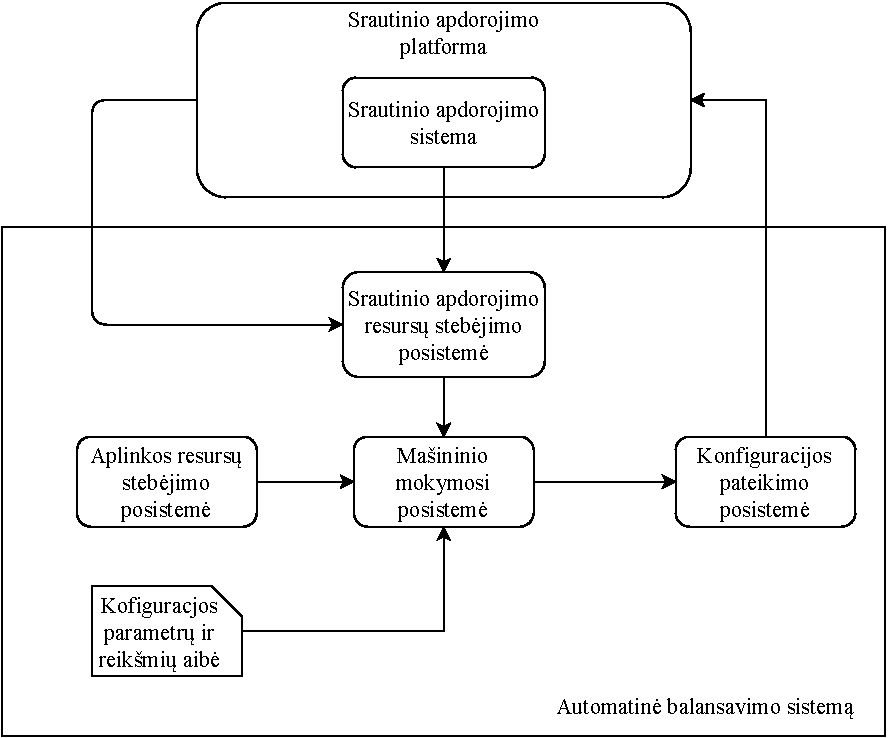
\includegraphics[width=15cm]{img/BalansavimoDiagrama.pdf}
    \caption{Pagrindiniai algoritmo elementai ir jų tarpusavio ryšiai}
    \label{balansavimo_sistema}
\end{figure} 

\subsection{Tikslas}
Algoritmo tikslas savarankiškai reguliuoti srautinio apdorojimo sistemos konfiguracijos parametrus siekiant palaikyti sistemą stablią ir optimaliai naudojančia resursus. \ref{balansavimo_sistema} pav. pavazduota sistema yra integruojama į srautinio apdorojimo sistemos platformą iš kurios ji gauna reikiamą informacija apie srautinio apdorojimo sistemos metrikas ir resursus, bei turėti informaciją apie esamus aplinkos naudojamus ir turimus resursus. Balansavimo algoritmas eksperimente bus implementuojamas kaip posistemė, kuri gauna metrikas iš srautinio apdorojimo sistemos platformos ir operacinės sistemos, o atnaujintą konfiguraciją pateikia į srautinio apdorojimo platformą per komandų įvedimo eilutę.

\subsection{Įeiga}
Kad mašinio mokymosi posistemė galėtų daryti sprendimus, jai paduodami šie duomenys:
\begin{itemize}
    \item Srautinio apdorojimo sistemos naudojami resursai ir metrikos – procesoriaus apkrova, operatyviosios atminties apkrova, priešslėgis (angl. backpressure), srautinio apdorojimo sistemos įeigos komponento atsilikimas nuo duomenų srauto.
    \item Aplinkos naudojami resursai – procesoriaus apkrova, operatyviosios atminties apkrova.
    \item Srautinio apdorojimo sistemos pradinė konfiguracija – komponentų lygiagretumo parametrai, konteinerių parametrai, konfiguracijos elementai ir jų reikšmės.
    \item Konfiguruojami parametrai ir jų reikšmių ribos.
    \item Mašinio mokymosi algoritmo konfiguracija – sprendimų priemimo periodiškumas.
\end{itemize}

\subsection{Eiga}

Sistema naudojanti mašininį mokymąsi veikia pastoviai vienodo periodo ciklais (\ref{veikimas} pav.). 
\begin{figure}[H]
    \centering
    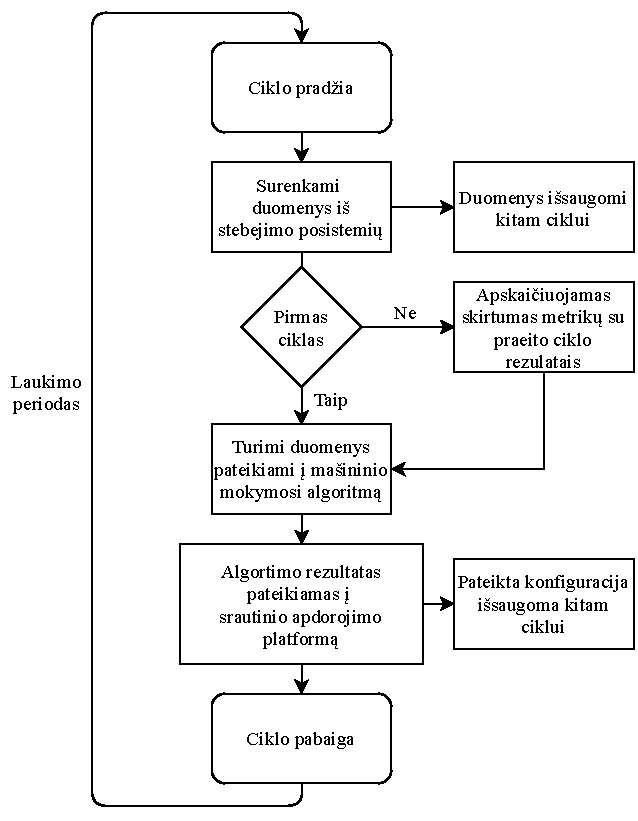
\includegraphics[width=10cm]{img/AlgoritmoVeikimas.pdf}
    \caption{Algortimo veikimas}
    \label{veikimas}
\end{figure} 
Tarpas tarp ciklų apibrežiamas leidžiant balansavimo sistemai ir yra skirtas srautinio apdorojimo sistemai atsinaujinti su naujais konfiguracijos parametrais bei kad surinkti duomenys būtų pakankamai svarūs pateikti į mašininį mokymosi algoritmą.
Tarp ciklų taip pat yra renkamos metrikos apie būseną, kurie bus veliau paduodami mašininio mokymosi algoritmui.

\subsection{Algoritmo rezultatas}
Mašinio mokymosi posistemė, atlikusi skaičiavimus, gražiną naują konfiguracijos parametrų rinkinį, kuris yra veliau pateikiamas į srautinio apdorojimo sistemų platformą. Po srautinės apdorojimo sistemos pradedamas naujas ciklas sistemos stebėjimo ir naujų konfiguracijos parametrų kurimo, kuris taip pat atsižvelgia į metrikų skirtumo ir konfiguracijos pakeitimo rezultatus iš  ankstesnių ciklų.

\sectionnonum{Išvados}

\printbibliography[heading=bibintoc] 

\end{document}
